\documentclass[12pt]{article}
\usepackage[margin=1in]{geometry}
\usepackage{graphicx}
\usepackage{float}
\usepackage{amsmath}
\usepackage{amsfonts}
\usepackage{amssymb}
\usepackage{booktabs}
\usepackage{pgfplots}
\pgfplotsset{compat=1.17}

\title{Sampling and Quantization Problems}
\author{Sean Balbale}
\date{November 26, 2024}

\begin{document}

\maketitle
\newpage

\section{Problem 1: A/D Converter with Full-Scale Range of ±10V}
\subsection*{(a) Resolution of the A/D}
The resolution of the A/D converter is given by:
\[
\text{Resolution} = \frac{\text{Full-scale range}}{\text{Number of levels}}
\]
For a 3-bit A/D converter, the number of levels is \(2^3 = 8\). Thus:
\[
\text{Resolution} = \frac{20}{8} = 2.50 \, \text{V}
\]

\subsection*{(b) Maximum Quantization Error}
The maximum quantization error is half of the resolution:
\[
\text{Maximum Error} = \frac{\text{Resolution}}{2} = \frac{2.50}{2} = 1.25 \, \text{V}
\]

\subsection*{(c) Quantization Levels}
The quantization levels for a 3-bit A/D converter with a range of ±10 V are:
\[
-8.75, -6.25, -3.75, -1.25, 1.25, 3.75, 6.25, 8.75 \, \text{V}
\]

\begin{figure}[H]
    \centering
    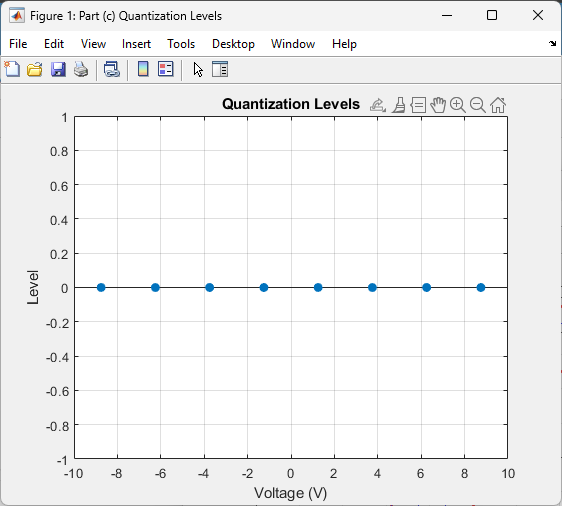
\includegraphics[width=0.7\textwidth]{C_Sketch.png}
    \caption{Quantization Levels for 3-bit A/D Converter.}
    \label{fig:quantization}
\end{figure}

\subsection*{(d) Expression for Discrete-Time Signal}
The discrete-time signal is given by:
\[
x[n] = x(nT_s) = 5 \sin(2000\pi nT_s)
\]
The sampling interval \(T_s\) is:
\[
T_s = \frac{1}{F_s} = \frac{1}{8000} = 0.000125 \, \text{s}
\]
The discrete-time frequency \(\Omega\) is:
\[
\Omega = 2\pi f T_s = 0.25\pi \, \text{radians/sample}
\]

\subsection*{(e) Minimum Sampling Frequency}
The Nyquist theorem states:
\[
F_s \geq 2f_{\text{max}}
\]
For \(f_{\text{max}} = 1000 \, \text{Hz}\), the minimum sampling frequency is:
\[
F_s = 2000 \, \text{Hz}
\]

\subsection*{(f) Quantized Signal}
The samples and quantized signal are shown in Figure~\ref{fig:quantized_signal}.
\begin{figure}[H]
    \centering
    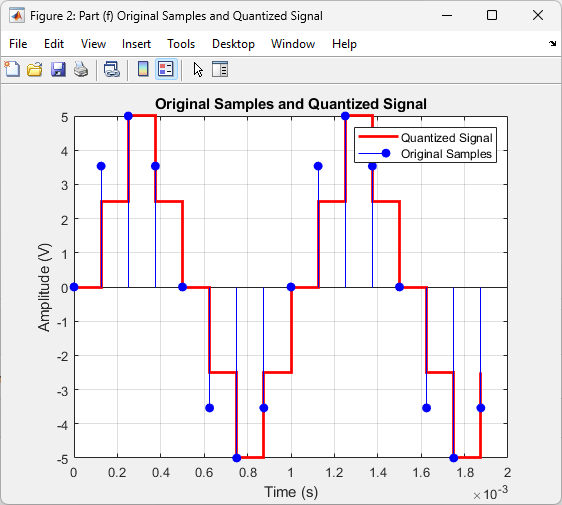
\includegraphics[width=0.7\textwidth]{F_Sketch.png}
    \caption{Original Samples and Quantized Signal.}
    \label{fig:quantized_signal}
\end{figure}

\section{Problem 2: Signal with Peak Values of ±0.2V}
\subsection*{(a) Minimum Number of Bits Without Amplification}
Quantization error should not exceed 0.1\% of the maximum signal amplitude (\(A = 0.2\)):
\[
\text{Error} = 0.001 \times A = 0.0002 \, \text{V}
\]
The resolution must be less than or equal to \(0.0002 \, \text{V}\):
\[
\text{Resolution} = \frac{\text{Full-scale range}}{2^N} \implies 2^N \geq \frac{5}{0.0002} = 25000
\]
Thus, \(N \geq 15\).

\subsection*{(b) Minimum Sampling Frequency}
The Nyquist theorem gives:
\[
F_s \geq 2f_{\text{max}} = 2 \times 4000 = 8000 \, \text{Hz}
\]

\subsection*{(c) Amplified Signal}
The gain factor required to extend the signal range from ±0.2V to ±5V is:
\[
\text{Gain} = \frac{5}{0.2} = 25
\]
With amplification, the resolution is recalculated:
\[
2^N \geq \frac{5}{0.0002} \implies N \geq 10
\]

\section{Problem 3: Composite Waveform}
\subsection*{(a) Minimum Sampling Rate}
The highest frequency component is \(1000 \, \text{Hz}\). Thus:
\[
F_s \geq 2 \times 1000 = 2000 \, \text{Hz}
\]

\subsection*{(b) Quantization Levels}
The number of quantization levels for a 10-bit system is:
\[
2^{10} = 1024
\]

\subsection*{(c) Maximum Quantization Error}
The resolution is:
\[
\text{Resolution} = \frac{20}{1024} = 0.01953 \, \text{V}
\]
The maximum quantization error is half the resolution:
\[
\text{Error} = \frac{0.01953}{2} = 0.00977 \, \text{V}
\]

\subsection*{(d) Storage Requirement}
For a 4 kHz sampling rate over 10 minutes:
\[
\text{Samples} = F_s \times \text{time} = 4000 \times (10 \times 60) = 2400000
\]

\subsection*{(e) New Signal}
For \(f_{\text{max}} = 2500 \, \text{Hz}\), the new sampling rate is:
\[
F_s = 5000 \, \text{Hz}
\]
The quantization levels and maximum error remain unchanged.

\section{Problem 4: Audio Signal Sampling}
\subsection*{(a) Original Frequencies}
The original frequencies present in \(x(t)\) are:
\[
1000 \, \text{Hz}, 1500 \, \text{Hz}, 3000 \, \text{Hz}
\]

\subsection*{(b) Discrete-Time Frequencies}
The discrete-time frequencies are:
\[
\Omega = \{1.57, 2.36, -1.57\} \, \text{radians/sample}
\]

\subsection*{(c) Reconstructed Frequencies}
The reconstructed frequencies are:
\[
1000 \, \text{Hz}, 1500 \, \text{Hz}
\]
These match the audible frequencies in the original signal.

\end{document}
